\documentclass[12pt]{article}
\usepackage[margin=1in]{geometry}

% PACKAGES
\usepackage{amsmath} % For extended formatting
%\usepackage{amssymb} % For math symbols
\usepackage{amsthm} % For proof environment
\usepackage{array} % For tables
\usepackage{enumerate} % For lists
\usepackage{extramarks} % For headers and footers
\usepackage{fancyhdr} % For custom headers
\usepackage{graphicx} % For inserting images
\usepackage{multicol} % For multiple columns
\usepackage{verbatim} % For displaying code
%\usepackage{tkz-euclide}
\usepackage{pgfplots}
\usepackage{tasks}

% SET UP HEADER AND FOOTER
\pagestyle{fancy}
\lhead{\MyCourse} % Top left header
\chead{\MyTopicTitle} % Top center header
\rhead{\MyAssignment} % Top right header
\lfoot{\MyCampus} % Bottom left footer
%\cfoot{June 14, 2022} % Bottom center footer
\rfoot{\MySemester} % Bottom right footer
\renewcommand\headrulewidth{0.4pt} % Size of the header rule
\renewcommand\footrulewidth{0.4pt} % Size of the footer rule
\setlength{\headheight}{14.49998pt}

\let\ds\displaystyle
\newcommand{\red}{\textcolor{red}}
\newcommand{\blue}{\textcolor{blue}}
\newcommand{\pink}{\textcolor{CarnationPink}}
\newcommand{\orange}{\textcolor{orange}}
\newcommand{\purple}{\textcolor{purple}}
\newcommand{\violet}{\textcolor{violet}}
\newcommand{\cyan}{\textcolor{cyan}}
\newcommand{\grn}{\textcolor{green}}
\newcommand{\uh}{\textcolor{ForestGreen}}

% ----------
% TITLES AND NAMES 
% ----------

\newcommand{\MyCourse}{Math 242}
\newcommand{\MyAssignment}{Worksheet 13}
\newcommand{\MySemester}{Fall 2024}
\newcommand{\MyCampus}{University of Hawaii at Manoa}


\pgfplotsset{compat=1.18} 
\begin{document}
\noindent Name: \hspace{4in}Section:
\vspace{0.5cm}



\begin{enumerate}
\item Show that every member of the family of functions $y=(\ln{x}+C)/x$ is a solution of the differential equation $x^2y'+xy=1$.
\vfill
\item Select a direction field for the differential equation $y'=y^2-x^2$ from the set of direction fields shown below.\\
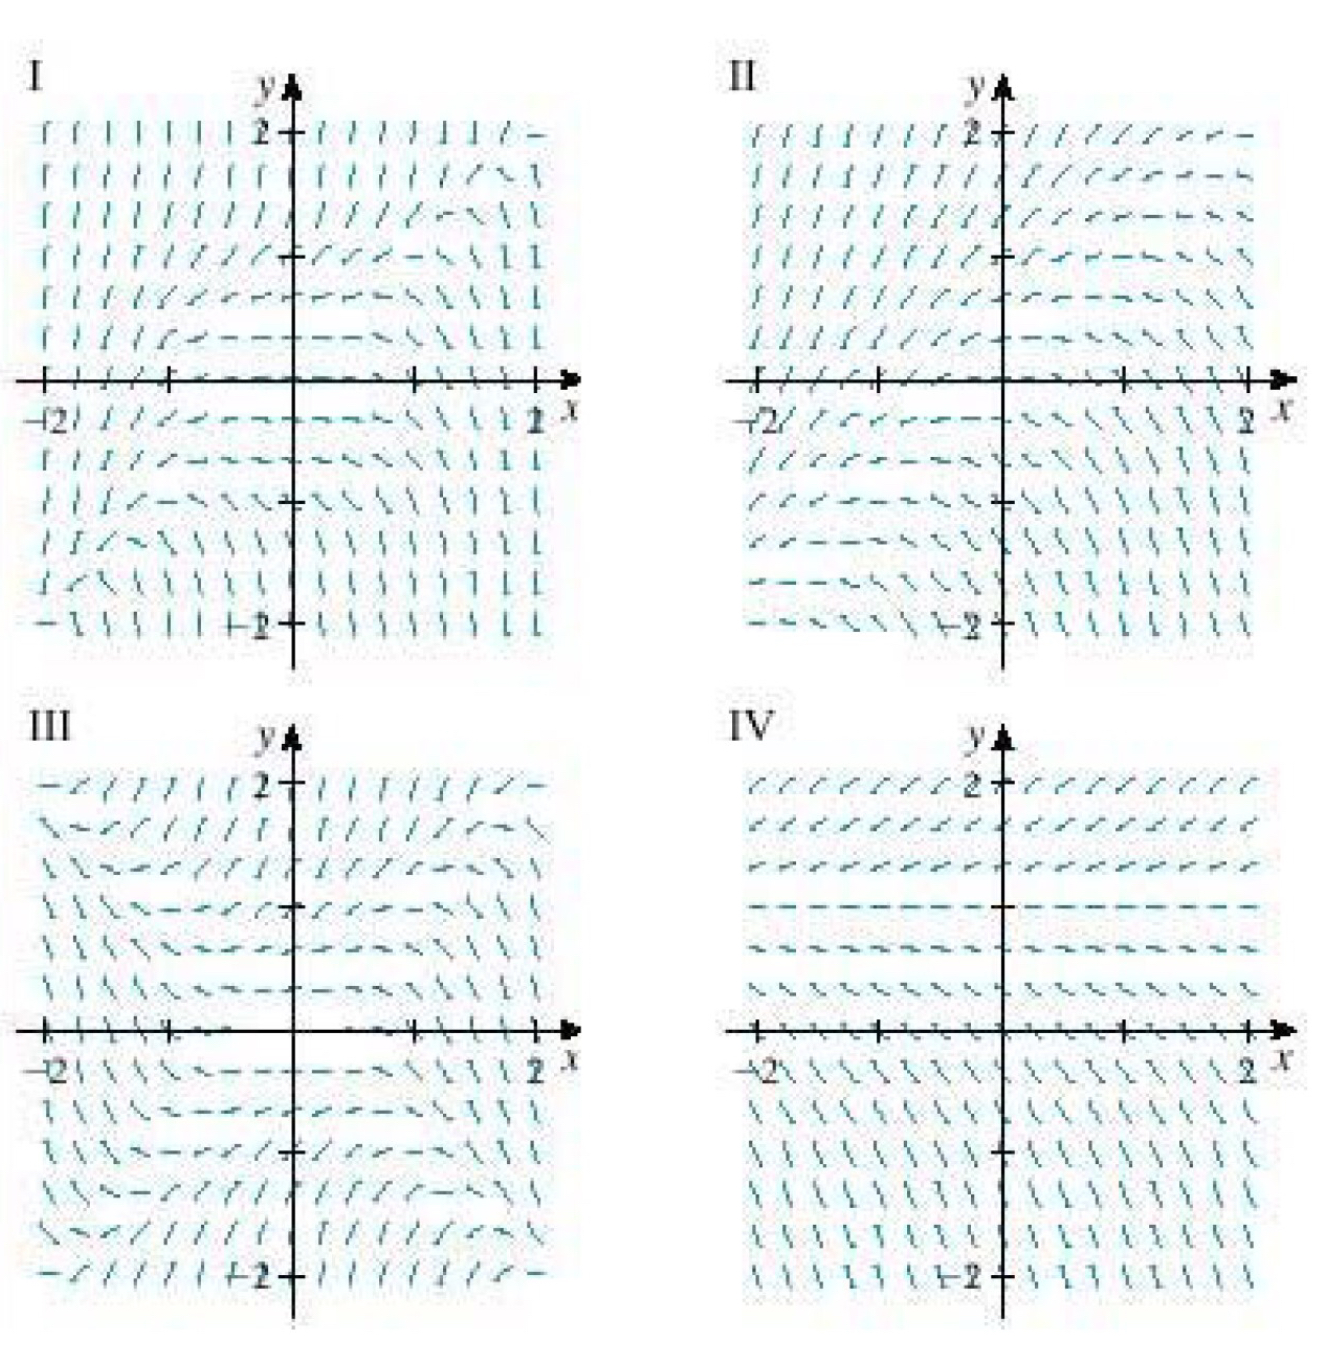
\includegraphics[width=10cm]{IMG_2808.jpg}
\newpage
\item Choose the differential equation corresponding to this direction field.\\
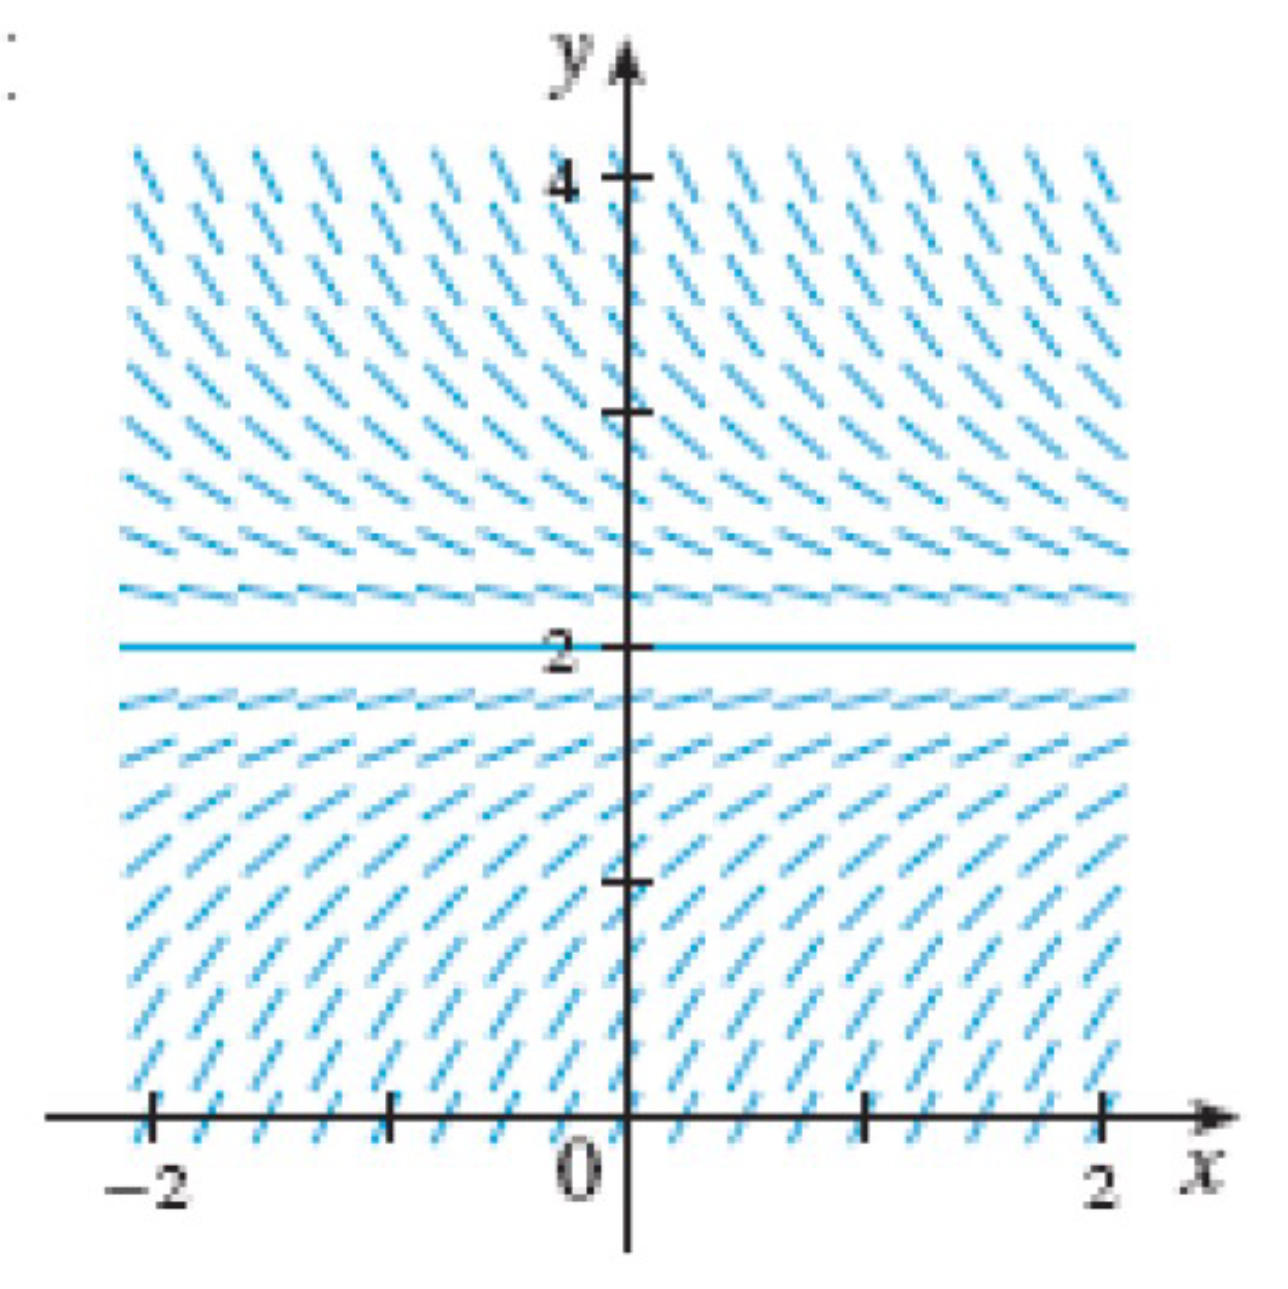
\includegraphics[width=7cm]{IMG_2807.jpg}
\begin{enumerate}
    \item $y'=\sin{x}\sin{y}$
    \item $y'=2-y$
    \item $y'=x+y-1$
    \item $y'=y+xy$
    \item $y'=x(2-y)$
\end{enumerate}
\item Find the solution of the differential equation $x+3y^2\sqrt{x^2+1}\frac{dy}{dx}=0$ that satisfies the  initial condition $y(0)=1$.
\vfill
\newpage
\item Find the orthogonal trajectories of the family of curves: $x^2-y^2=k$
\vfill
\item Roughly sketch the direction field for the differential equation given by $\frac{dy}{dt}=y-t$ with initial value $y(0)=1$ and $y(1)=-2$.
\vfill

\end{enumerate}


\end{document}